\documentclass{article}
\usepackage[utf8]{inputenc}

\usepackage{amsfonts}
\usepackage{enumitem}
\usepackage{amsmath}
\usepackage{xcolor}
\usepackage{hyperref}
\usepackage{graphicx}
\graphicspath{ {Figs/} }

\hypersetup{
    colorlinks=true,
    linkcolor=blue,
    filecolor=magenta,      
    urlcolor=cyan,
    pdftitle={Overleaf Example},
    pdfpagemode=FullScreen,
    }


\usepackage{geometry}
\geometry{margin=0.75in}



\begin{document}
\title{CMPSCI 389 Final Project Milestone 2 (HW6)}
\author{\textbf{YOUR NAME(s) HERE}}
\date{Assigned: April 23nd 2024; Due: April 30th 2024 @ 11:59 pm EST}

\maketitle

\begin{abstract}
    So now we're in the home stretch -- it's time for you to show off all of the work you've been pouring into your projects. Or it's time for you to scramble to get something together so that you manage to pass this class while also studying for finals. Either way, welcome to milestone 2! \\ \\
    \textbf{The final demos will be in class on May 15th}, so I hope this keeps you on track for that. You'll also need to put together a video demo for it by May 17th so get ready for that too! BTW, you should submit these in your groups, so hope you don't hate them yet!
    
\end{abstract}

\section{New results (35 points)}

Now that you know exactly what your final project is you have a whole extra week to get some new results. Just like last time, I want you to show some graphs/images of you progress. You can include whatever you have done (not code), but I expect 3 \textit{different} images that are higher quality than last time (label your axes and graph!). This homework doesn't have much you need to write, this is to give you time to produce some good stuff here, so use that time!


\begin{figure}[htb]
    \centering
    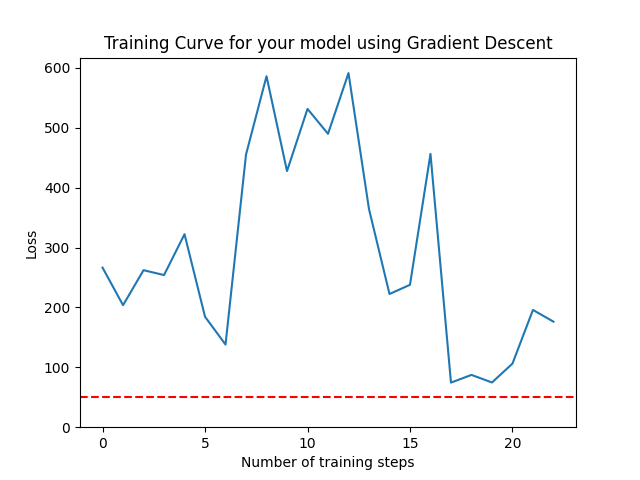
\includegraphics[width=0.4\textwidth]{Figs/Example training.png}
    \caption{ Example caption}
    \label{fig:net}
\end{figure}

\section{Result explanation (20 points)}

Here I want you to give detailed explanations of how you produced each graph and what the results of each mean. The results don't necessarily have to be good (though that's better) but the explanation has to be! You can combine this and the previous section so that the explanations go with the images if that is natural for you.

\section{Plan for Demos (25 points)}

You'll have to both give a demo in class and make a demo video of your project. In this section I want you to plan out both of these. Please include how each demonstration will work, what you'll show, and write a short synopsis of your explanation (the motivation, model setup, dataset used, etc ). Please do this part as a team!

\section{The bit where you can rant (15 points)} \textbf{Do this part after everything else.} In this part I want to hear what went well, what went okay and what didnt. List off 3 things that have gone well through this project so far, 3 things that you would do differently in hindsight. This is less important for me than it is for you -- I want you to be able to reflect that starting last minute or trying to invent AGI was a mistake.  

\end{document}